%%%%%%%%%%%%%%%%%%%%%%%%%%%%%%%%%%%%%%%%%%%%%%%%%%%%%%%%%%%%%%%%%%%%%%%%%%%%%%%%
%2345678901234567890123456789012345678901234567890123456789012345678901234567890
%        1         2         3         4         5         6         7         8

\documentclass[letterpaper, 10 pt, conference]{ieeeconf}  % Comment this line out
                                                          % if you need a4paper
%\documentclass[a4paper, 10pt, conference]{ieeeconf}      % Use this line for a4
                                                          % paper

\IEEEoverridecommandlockouts                              % This command is only
                                                          % needed if you want to
                                                          % use the \thanks command
\overrideIEEEmargins
% See the \addtolength command later in the file to balance the column lengths
% on the last page of the document



% The following packages can be found on http:\\www.ctan.org
\usepackage{graphicx} % for pdf, bitmapped graphics files
\usepackage{epsfig} % for postscript graphics files
\usepackage{mathptmx} % assumes new font selection scheme installed
\usepackage{times} % assumes new font selection scheme installed
%\usepackage{amsmath} % assumes amsmath package installed
%\usepackage{amssymb}  % assumes amsmath package installed
\usepackage{subfigure}  % postscript figures
\usepackage{url}        % \url{} command with good linebreaks
\usepackage {cite}
\usepackage {algorithmic}
\usepackage {algorithm}
\usepackage {setspace}

\title{\LARGE \bf
Experimental results under the bare-bone network
}

\author{Ju-Young Jung and Jonghoon Choi% <-this % stops a space
	\\\textit{University of Pittsburgh}%
	\\\textit{\{juyoung@cs.pitt.edu, joc66@pitt.edu}\}
}

\begin{document}

\maketitle
\thispagestyle{plain}
\pagestyle{plain}


%%%%%%%%%%%%%%%%%%%%%%%%%%%%%%%%%%%%%%%%%%%%%%%%%%%%%%%%%%%%%%%%%%%%%%%%%%%%%%%%
\section{Measurement under infinite queue size}
\label{sec:exp1}
\noindent 
In the first experiments, we measured average end-to-end delay and rate of packets
that arrive later than 150 ms, which is the end-to-end delay constraints, 
under bottoleneck bandwidth at 100 Kbps, 500 Kbps and 1 Mbps, respectively.\\

\subsection{\bf{Measure average End-to-End delay with infinite queue size}}
\label{sec:EEDdelay_Inf}

\begin{figure}[t]
\centering
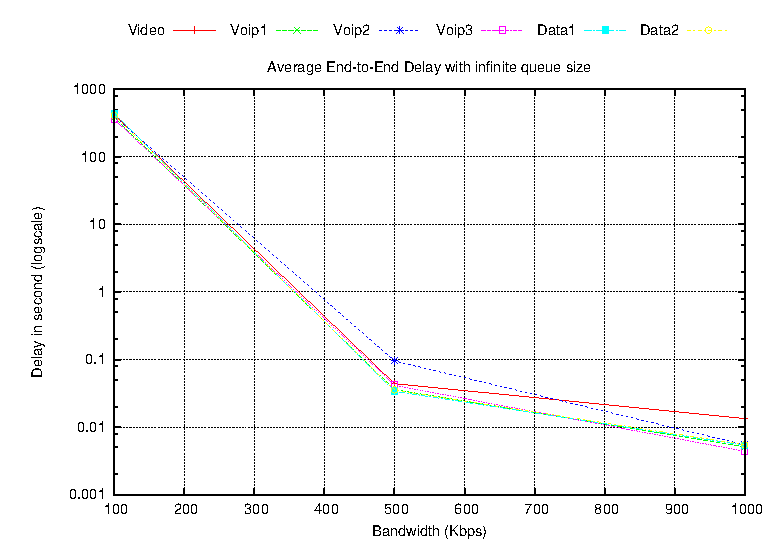
\includegraphics{./graphs/AvgEED.eps}
\caption{
Average end-to-end delay with infinite queue size (=20000)
}
\label{fig:AvgEED}
\end{figure}

\noindent
First, we define 20000 of queue size as the infinite queue size since there is no different
result with larger queue size than 20000.\\

As we expected, we can observe that the higher bandwidth, the lower delay.
Since we used the infinite queue, there is no dropped packet.
As a result, the end-to-end delay expoenentaily increases at lower bandwidth.

\subsection{\bf{Measure rate of packets that do not arrive on time (150 ms)}}
\label{sec:Laterate}
\noindent 

\begin{figure}[t]
\centering
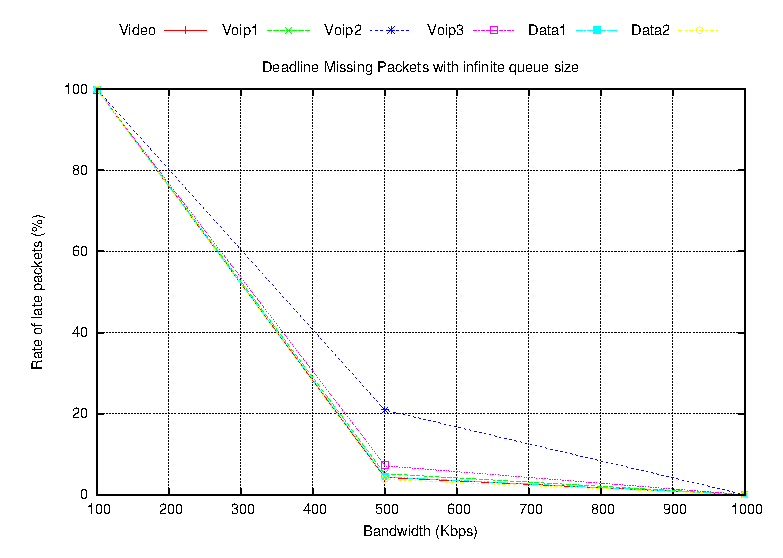
\includegraphics{./graphs/deadlineEED.eps}
\caption{
Rate of packets that violoate end-to-end delay constraints
}
\label{fig:deadlineEED:}
\end{figure}

\section{Experiments with varying queue size}
\label{sec:exp2}
\noindent 
In the second experiments, 


First, we adjust the value 

\end{document}
% test
